\documentclass[11pt, a4paper, twoside]{montblanc2}
\usepackage[T1]{fontenc}
\usepackage{url}
\usepackage{color}
\usepackage{xspace}
\usepackage{listings}
\usepackage{graphics}

\def\cmake{\textsc{CMake}\xspace}
\def\lua{\textsc{Lua}\xspace}
\def\dd{\textsc{DwarfDump}\xspace}
\def\elfutils{\textsc{ElfUtils}\xspace}

\urlstyle{sf}

\definecolor{bluelst}{rgb}{0.4,0.8,1.0}
\definecolor{greenlst}{rgb}{0.25,0.50,0}

\lstdefinestyle{C}{
  language=C,
  basicstyle=\small\sffamily,
  frame=single,
  rulecolor=\color{bluelst},
  commentstyle=\color{greenlst}\textit,
  keywordstyle=\bfseries,
  breaklines=true,
  numbers=left,
  numberstyle=\tiny,
  numbersep=5pt,
  tabsize=4
}

\lstdefinestyle{BOAST}{
  language=Ruby,
  basicstyle=\small\sffamily,
  frame=single,
  rulecolor=\color{bluelst},
  commentstyle=\color{greenlst}\textit,
  keywordstyle=\bfseries,
  breaklines=true,
  numbers=left,
  numberstyle=\tiny,
  numbersep=5pt,
  tabsize=2,
  morekeywords={BOAST, pr, decl, opn, close}
}

\begin{document}
\devnum{[5.11]}
\title{[MAQAO in BOAST]}
\version{[0.1]}
\deadline{[2017/01/16]}
\level{[PU]}
\nature{[O]}
\authors{Olivier Aumage (Inria) and Brice Videau (CNRS)}
\contributors{} % {Name (PARTNER), Name (PARTNER), Name (PARTNER)}
\reviewers{} % {Name (PARTNER), Name (PARTNER), }
\keywords{[analysis, autotuning, performance]}

\maketitle

\begin{changelog}
\change{0.1}{Initial version of D5.11}
\end{changelog}

\frontmatter

\begin{executive}
  \todo{executive summary}
\end{executive}

\section{Introduction}
\todo{intro}

\section{Context}
\todo{context}

\subsection{BOAST}
\begin{itemize}
  \item General presentation of BOAST
  \item Purpose, capabilities, usage
\end{itemize}

\lstdefinestyle{Bash}{
  language=Bash,
  basicstyle=\small\sffamily,
  frame=single,
  rulecolor=\color{bluelst},
  commentstyle=\color{greenlst}\textit,
  keywordstyle=\bfseries,
  breaklines=true,
  numbers=left,
  numberstyle=\tiny,
  numbersep=5pt,
  tabsize=4
}

\subsubsection{Presentation}

BOAST is an automatic performance tuning framework aiming at meta-programming and optimizing computing kernels.
BOAST has been extensively described in the Mont-Blanc 2 deliverable 5.5~\cite{tichadou15} and thus will only be briefly described here.
For a more in-depth presentation, reader should refer to the afore mentioned document.

The primary goal of BOAST is to bring performance portability to critical parts of high performance computing applications.
Those \emph{computing kernels} are well-defined parts of an application that are compute or memory intensive and represent a significant part of the computing time.
Their inputs are usually limited in complexity, thus those kernels are a prime target for optimization.

Unfortunately, the variety of platforms an HPC code can encounter keeps growing, and a lot of time is spent optimizing computing kernels for new architectures.
BOAST attempts to solve this problem by offering the kernel developer several tools:
\begin{itemize}
  \item an Embedded Domain Specific language to describe computing kernels and their possible optimizations;
  \item a code generation engine that can output the kernel in several languages used in the HPC community: C, FORTRAN, CUDA and OpenCL;
  \item a runtime to select the versions to test, build them, execute them and test their performance and accuracy.
\end{itemize}


\subsubsection{Usage}


The usage of BOAST will be illustrated using the following Ruby/BOAST listing.
This example shows how to load BOAST, change it's environment, define a simple vector addition kernel, execute it using different languages, and check the accuracy of the obtained results.

\lstset{style=BOAST}
\begin{lstlisting}
require 'BOAST'
include BOAST

set_array_start(0)
set_default_real_size(4)

def vector_add
  n = Int( "n", :dir => :in)
  a = Real("a", :dir => :in,  :dim => [ Dim(n) ] )
  b = Real("b", :dir => :in,  :dim => [ Dim(n) ] )
  c = Real("c", :dir => :out, :dim => [ Dim(n) ] )
  p = Procedure("vector_add", [n,a,b,c]) {
    decl i = Int("i")
    expr = c[i] === a[i] + b[i]
    if (get_lang == CL or get_lang == CUDA) then
      pr i === get_global_id(0)
      pr expr
    else
      pr For(i,0,n-1) {
        pr expr
      }
    end
  }
  return p.ckernel
end

n = 1024*1024
a = NArray.sfloat(n).random
b = NArray.sfloat(n).random
c = NArray.sfloat(n)

c_ref = a + b
epsilon = 10e-15

[FORTRAN, C, CL, CUDA].each { |l|
  set_lang( l )
  puts "#{get_lang_name}:"
  k = vector_add
  puts k
  c.random!
  k.run(n, a, b, c, global_work_size: [n,1,1], local_work_size: [32,1,1])
  diff_max = (c_ref - c).abs.max
  raise "Error: max error too big: #{diff_max}!" if diff_max > epsilon
}
puts "Success!"
\end{lstlisting}

\paragraph{Loading BOAST} is done on lines 1 and 2.
It loads the BOAST framework in its environmental configuration.
This configuration can be changed through configuration files or environment variables.
Here, this configuration is changed on lines 4 and 5 to set the default real variable size to 4 bytes and the first index of arrays to 0 (C like arrays).

\paragraph{Kernel definition} is done on lines 7 to 25.
The definition is enclosed in a procedure that will be called in different contexts, yielding different kernel versions.
First, the parameters of the kernel are defined on lines 8 to 11, and stored in ruby variables.
Those parameters have a direction (similar to FORTRAN intent). The \emph{Real} parameters have a dimension, meaning they are arrays, in this case of length \emph{n}.
The \emph{Procedure} is declared on line 12 by giving its name and parameter list.
It is associated a block of code that spans from line 12 to 23 and constitute its body.
A local integer variable \emph{i} is defined on line 12 and declared using the keyword \emph{decl}.
On line 14, an assignment expression is saved for later use in the ruby variable \emph{expr}.
This expression computes one element of the result array.
The difference between a ruby assignment (using the \emph{=} operator) and a BOAST assignment (using the \emph{===} operator) has to be noted.
On lines 15 to 22 we can see some BOAST meta-programming.
Here, based on the BOAST \emph{lang} state, the code will select either a GPU or CPU implementation.
The GPU implementation obtains an index of the element to process (line 16) and stores it into the \emph{i} variable.
This is printed using the \emph{pr} keyword, meaning that this line is to appear in the generated source.
The expression we saved earlier is then printed (line 17).
The CPU implementation prints a for loop that will process all the elements of the arrays.
We can see here an example, though far-fetched, of code factoring.
The line 24 returns the computing kernel object corresponding to the printed \emph{p} procedure.
The procedure \emph{vector\_add} is automatically set as the entry point of the computing kernel.

\paragraph{Kernel execution} is done on lines 27 to 48.
Line 27 to 30 define input values for our kernel.
Three of these objects are numerical arrays of size \emph{n}, two of them (input ones) are initialized with random values.
A reference result is computed on line 32.
An epsilon is defined to check the accuracy of further computed results (line 33).
From line 35 to 44 the kernel will be generated for each target language supported by BOAST.
To do this we first change the BOAST \emph{lang} state and print it on the standard output (lines 36 and 37).
The \emph{vector\_add} ruby procedure is then called, which generates a new instance of the computing kernel, adapted to the chosen language (line 38).
The generated code is then printed to the standard output.
The output array is set randomly and then the computing kernel is called through the \emph{run} method  (line 44).
Compilation is launched implicitly here, it could also be requested explicitly by calling the \emph{build} method.
First, the kernel takes positional arguments that correspond to its parameters.
The following parameters are named options that are ignored in \emph{C} and \emph{FORTRAN} but interpreted in \emph{OpenCL} and \emph{CUDA}.
Once the kernel has finished executing we compare the output \emph{c} to the computed reference (line 42) and raise an error should the maximum discrepancy be superior to \emph{epsilon}.

\paragraph{Installation} of BOAST is made through the simple following command provided ruby >= 1.9.3 and its development files are installed.

\lstset{style=Bash}
\begin{lstlisting}
gem install --user-install BOAST
\end{lstlisting}



\subsection{MAQAO}
%\begin{itemize}
%  \item General presentation of MAQAO
%  \item Purpose, capabilities, usage
%\end{itemize}

\subsubsection{Presentation}
MAQAO, the Modular Assembly Quality Analyzer and Optimizer, is a performance analysis and processing 
tool working at the level of compiled, binary code. It was initially developed at the University of 
Versailles in France, and has been partially developed at Inria in Bordeaux as well since around 
2010. While primarily focused on Intel processors (x86-64, xeon phi, and even Itanium), it was 
ported on the ARM architecture as part of Mont-Blanc~2 task D5.3 work, and delivered as 
Deliverable~D5.4. The MAQAO tool presents itself as an extensible framework for binary code 
processing. It is a made of a C-language low-level core set of libraries and a high-level set of 
wrappers making the framework scriptable in the language \lua using the embedded interpretor. 

The core libraries of MAQAO enable the fundamental operations to disassemble a binary file, modify 
its assembly instructions (operation designated as 'patching'), and re-assemble the modified binary. 
Possible instruction modifications include moving/inserting/suppressing code blocks, inserting 
function calls, or operations designated as 'instrumentation' where some sets of instructions are 
both moved and modified such as a function call is made every time such instructions are called 
before executing the instrumented instructions themselves. Core services also include foundational 
capabilities such as building call graphs and control flow graphs from the disassembled binary 
functions.

A set of \lua-to-C wrapper routines implement the transition between the C~core and the Lua 
services. These routines enable to manipulate relevant assembly objects such as binary files, 
functions, basic instruction blocks, individual instructions, instruction operands, loops and 
labels. 

On top of those transitional routines, special-purpose processing modules can be implemented in Lua 
to perform high level operations such as analysis, tracing and hinting. In particular, tracing 
involves instrumenting every memory reference in the studied kernel with calls to the memory access 
accounting routine in the MAQAO Trace Library (MTL) which monitor every memory address referenced 
within the kernel routine during an execution, and generate a compressed trace of the memory 
references. The trace can then be further processed to output memory access patterns as human 
readable algebraic expressions.

\subsubsection{Usage}

The MAQAO framework version developed in Bordeaux is very much targeted at an experimented audience, 
and, as a note of warning, it may lack the user friendliness commonly found in mature academic and 
commercial programming tools. It is aimed at expert users desirous to dig further into the binary 
kernel code produced by their compiler, and build their own, custom analysis strategies.
This section presents MAQAO from a functional point-of-view, and specify usage for the most common
operations.

\paragraph{Requirements and Installation}

MAQAO's C language core mandatorily requires \cmake version~2.8.8 or above, a C compiling toolchain 
and Make. The \lua layers directly make use of the embedded \lua distribution. Moreover, MAQAO 
analysis scripts may leverage the command-line tool \dd to process debugging informations and 
symbols in compiled objects files when available, while \dd itself relies on the availability of an 
\elfutils distribution. Supported binary objects and executables to be processed by MAQAO must 
follow the ELF format specification and System V general ABI specification, and be generated for the 
ARM architecture, while optional debugging information must follow the DWARF-2 format. Support for 
ARM's Thumb instruction sets is limited to disassembly only.

Building MAQAO involves running \cmake followed by the \verb|make| command after untaring the 
distribution or checking it out from the development repository:

\begin{verbatim}
$ tar zxf maqao.tar.gz
$ cd MAQAO
$ mkdir build
$ cd build
$ cmake -DARCHS=arm -DSTRIP=false ..
$ make
\end{verbatim}

No install step is required. MAQAO's executable is produced in \verb|MAQAO/bin| and MAQAO's 
libraries are placed in the \verb|MAQAO/lib| directory. MAQAO's \verb|/bin| and \verb|/lib|
directories should be added to \verb|PATH| and \verb|LD_LIBRARY_PATH| environment variables 
respectively. Environment variable \verb|MAQAO| should be set to MAQAO's top directory for 
convenience, and is assumed to be set accordingly in the remainder of the document.

\paragraph{Disassemble}

Disassembling and low level assembly management is handled by MAQAO's Madras module. Every MAQAO 
module is accessed by specifying its name as first argument of MAQAO. Module's arguments are then 
prepended after the module name. Binary disassembled listing can be obtained using Madras as 
follows:

\begin{verbatim}
$ maqao madras -d <BINARY>
...
bf4c <s1111>:
 [...] f0 45 2d e9  0xbf4c push   {r4, r5, r6, r7, r8, sl, lr}; [...]
 [...] 02 8b 2d ed  0xbf50 vpush  d8; [...]
 [...] 14 d0 4d e2  0xbf54 sub    sp, sp, #20 ; [...]
 [...] 94 0d 0f e3  0xbf58 movw   r0, #64916 ; [...]
 [...] 01 00 40 e3  0xbf5c movt   r0, #1 ; [...]
...
\end{verbatim}

\paragraph{Instrument}

Instrumentation is the process of inserting probes for a set of specific
assembler instructions such that every time such an instruction is encountered
during execution, some accounting probe function can be called to account for
that instruction. Instrumentation in MAQAO is provided by the Memory module,
to target memory referencing instructions, such as to extract memory access
patterns at run-time. The Memory module itself calls the Madras module under the
hood to perform the low-level assembly manipulation involved.

\begin{verbatim}
$ maqao memory -i -bin=<BINARY> -f=<FUNCTION_NAME> -m=unicore -tp==<TEMP_DIR>
\end{verbatim}

Argument \verb|-i| requests instrumenting. Argument \verb|-bin| specifies the
binary executable to instrument. The MAQAO ARM port does not support
instrumenting position independent code (PIC) currently, thus the binary file
cannot be a shared library. Argument \verb|-f| specifies the function to
instrument. Argument \verb|-m| specifies the execution model. Finally, argument
\verb|-tp| specifies the directory in which the resulting instrumented binary
and its companion \lua meta-data file are generated. The actual instrumentations 
probe functions are trace recording routines from the MAQAO Trace Library (MTL).

Example below show diff between a uninstrumented binary listing fragment and the 
corresponding instrumented assembly code. Instruction \verb|vldr s14, [r1]| at 
address \texttt{0xbe78} (and other memory referencing instructions as well, such 
as the next one) is replaced by a branch to an inserted instruction block 
generically named \verb|@_patchmov_@|, generated by Madras to perform the memory 
access accounting.
\begin{footnotesize}
\begin{verbatim}
...
be78: ed917a00 vldr    s14, [r1]             | be78: ea15387a b       55a068 <@_patchmov_@>
be7c: ed537a01 vldr    s15, [r3, #-4]        | be7c: ea153899 b       55a0e8 <@_patchmov_@+
be80: ee777a27 vadd.f32        s15, s14, s15   be80: ee777a27 vadd.f32        s15, s14, s15
be84: ee171a90 vmov    r1, s15                 be84: ee171a90 vmov    r1, s15
...
\end{verbatim}
\end{footnotesize}

The assembly fragment below show part of the \verb|@_patchmov_@| block inserted 
by Madras. This block residing in the newly created \texttt{.madras.code} ELF 
section in the executable file is immediately preceded by another newly created 
section named \texttt{.madras.plt} containing the corresponding Procedure 
Linkage Table (PLT) containing the procedure entries for the indirect jumps into 
the MAQAO Trace Library routines.

\begin{footnotesize}
\begin{verbatim}
...
   >
   > Disassembly of section .madras.plt:
   >
   > 0055a044 <.madras.plt>:
   >   55a044: e3a0ca08 mov     ip, #32768      ; 0x8
   >   55a048: e59cc440 ldr     ip, [ip, #1088] ; 0x4
   >   55a04c: e5bcf038 ldr     pc, [ip, #56]!  ; 0x3
   >   55a050: e3a0ca08 mov     ip, #32768      ; 0x8
   >   55a054: e59cc440 ldr     ip, [ip, #1088] ; 0x4
   >   55a058: e5bcf03c ldr     pc, [ip, #60]!  ; 0x3
   >   55a05c: e3a0ca08 mov     ip, #32768      ; 0x8
   >   55a060: e59cc440 ldr     ip, [ip, #1088] ; 0x4
   >   55a064: e5bcf040 ldr     pc, [ip, #64]!  ; 0x4
   >
   > Disassembly of section .madras.code:
   >
   > 0055a068 <@_patchmov_@>:
   >   55a068: e52d0004 push    {r0}            ; (st

   >   55a0a8: e10f0000 mrs     r0, CPSR
   >   55a0ac: e92d47ff push    {r0, r1, r2, r3, r4, 
   >   55a0b0: ed2d8b10 vpush   {d8-d15}
   >   55a0b4: e24dd014 sub     sp, sp, #20
   >   55a0b8: e3000007 movw    r0, #7
   >   55a0bc: e1a02001 mov     r2, r1
   >   55a0c0: e52d2004 push    {r2}            ; (st
   >   55a0c4: e49d1004 pop     {r1}            ; (ld
   >   55a0c8: ebffffe0 bl      55a050 <__bss_end__+0
   >   55a0cc: e28dd014 add     sp, sp, #20
   >   55a0d0: ecbd8b10 vpop    {d8-d15}
   >   55a0d4: e8bd47ff pop     {r0, r1, r2, r3, r4, 
   >   55a0d8: e12ff000 msr     CPSR_fsxc, r0
   >   55a0dc: e49d0004 pop     {r0}            ; (ld
   >   55a0e0: ed917a00 vldr    s14, [r1]
   >   55a0e4: eaeac764 b       be7c <s111+0x60>
...
\end{verbatim}
\end{footnotesize}

The job of the code inserted in \verb|@_patchmov_@| is basically to:
\begin{enumerate}
\item \texttt{55a068..55a0b4:} Save the current program state (registers);
\item \texttt{55a0c8..55a0c8:} Call the relevant MTL accounting routine with the 
memory address of the instrumented memory reference, register \texttt{r1} here, 
in the case of instruction \texttt{0xbe78}, by jumping to the corresponding PLT 
entry and from there to the actual accounting routine;
\item \texttt{55a0cc..55a0dc:} Restore the program registers;
\item \texttt{55a0e0:} Execute the original, moved memory referencing 
instruction \verb|vldr s14, [r1]|;
\item \texttt{55a0e4:} Branch back to the main program at address 
  \texttt{0xbe7c}, immediately following the instrumented location 
  \texttt{0xbe78}, to continue program execution (which fortuitously happens to 
  be a memory reference also, and is thus instrumented as well).
\end{enumerate}

\paragraph{Trace}

Executing the resulting instrumented kernel produces a trace file containing a 
compressed representation of the target addresses of the memory accesses 
instruction encountered during execution. For each instruction instrumented, the 
flow of addresses captured is compressed on-the-fly using a lossless
algorithm name \emph{Nested Loop Recognition} (NLR), designed by Ketterlin and 
Clauss~\cite{ketterlin:nlr:cgo:2008}. The trace is stored using a compact text 
file format, not meant to be read as is by the programmer, as shown below.

\begin{footnotesize}
\begin{verbatim}
D 1 E 10 R 1 I 1 K 0 V  L P 39 L P 259 0 T 1 P 1262052 0 8 0 N N N I 2 K 0 V  L 
P 39 L P 259 0 T 1 P 3439840 0 8 0 N N N I 3 K 0 V  L P 39 L P 259 0 T 1 P 
3439852 0 8 0 N N N I 4 K 0 V  L P 39 T 1 P 3199305884 0 N N I 5 K 0 V  L P 39 T 
1 P 3199305888 0 N N I 6 K 0 V  L P 39 T 1 P 3199305892 0 N N I 7 K 0 V  L P 39 
T 1 P 3199305896 0 N N I 8 K 0 V  L P 39 L P 259 0 T 1 P 1262052 0 8 0 N N N I 9 
K 0 V  L P 39 L P 259 0 T 1 P 3439840 0 8 0 N N N I 10 K 0 V  L P 39 L P 259 0 T 
1 P 3439852 0 8 0 N N N 
\end{verbatim}
\end{footnotesize}

This intermediate format can however be processed by MAQAO's Memory module to 
produce a human-readable version of the NLR trace. The command below produces
the human-readable form of the trace from the compact trace and from the companion
\lua meta-data file generated during the instrumentation step.
 
\begin{verbatim}
$ maqao memory -d -t=<COMPACT_TRACE> -meta=<META_LUA_FILE> -tp=<TEMP_DIR>
\end{verbatim}

 This human-readable version shows, for each instrumented instruction, the
 corresponding thread id, the id of the loop containing the instruction as
 assigned by MAQAO, and the 'instrumented instruction' id also incrementally
 assigned by MAQAO. Multiple instances may exist when multiple threads invoke
 the instruction.

\begin{footnotesize}
\begin{verbatim}
Info: ################################################################################
Info: ## Volume for tid = 0 loopid = 21 iid = 0
Info: ################################################################################
Info: Instance 0
Info: ###############
for i0 = 0 to 39
  for i1 = 0 to 259
    val 0x1341e4 + 8*i1

 [...]
\end{verbatim}
\end{footnotesize}

Then, following the identification information, the successive values captured
by the instrumentation are represented by as a pseudo source-code with loops and
expressions. The expressions describe the memory addresses that have been
accessed, and depend on the surrounding loop counters and loop bounds, as
detected by the NLR algorithm. The portion of trace above corresponds to the
\texttt{b} array reference in the basic loop nest below extracted from routine
\texttt{s111} of the TSVC benchmark
suite~\cite{maleki:vectorization:pact:2011,callahan:tsvc:sc:1988}. Array
elements are 32-bit single precision floating point values. Thus, the
\texttt{8*i1} expression in the trace expresses a 2-element stride array
traversal corresponding to the innermost loop \texttt{i} index step value in the
source code. The \texttt{i0} is not referenced in the expression, meaning the
outer loop is a repetition loop.

\lstset{style=C}
\begin{lstlisting}
/* TSVC s111 kernel */
for (int nl = 0; nl < 2*ntimes; nl++) {
	for (int i = 1; i < LEN; i += 2) {
		a[i] = a[i - 1] + b[i];
	}
}
\end{lstlisting}

Trace expressions can, however, only depend linearly on the loop counters, and
loop bounds only depend linearly on enclosing loops' counters. The memory
addresses referenced by an expression forms an union of polytopes. Thus, the
method captures the memory working-set as well as a schedule for the memory
accesses.

\paragraph{Analyze}

MAQAO's SIMD analyzer is a MAQAO module built on top of the \lua API to analyze
simdization potential in compiled kernel binaries, as well as possible issues
hindering vectorization. The SIMD analyzer module can be applied to a kernel
using the following command:

\begin{verbatim}
export MAQAO_SA_PATH=$MAQAO/sa_analysis
maqao ${MAQAO_SA_PATH}/simd_analyzer.lua --dd <BINARY>:<FUNCTION>
\end{verbatim}

Flag \texttt{--dd} is optional, it assumes \dd is available on the system. When
enabled, the SIMD analyzer uses \dd to translate binary addresses into source
locations, provided the binary was compiled with debugging information included
(typically enabled by specifying the '-g' flag at compile time to the compiler).

% s1116
\begin{figure}[h]
  \centering
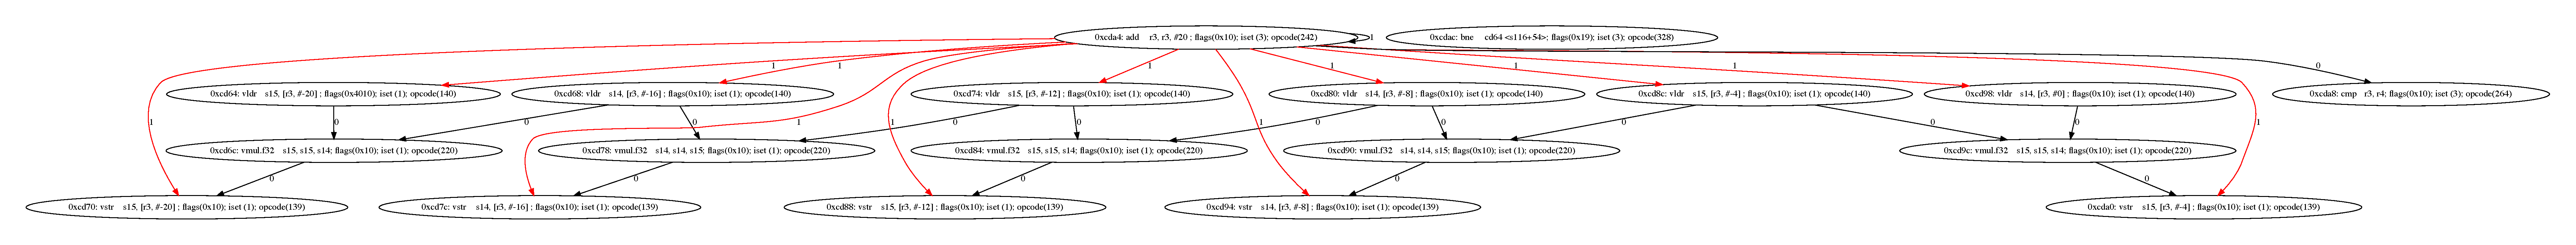
\includegraphics[width=1\textwidth]{fs116_l47}
\caption{Control flow graph for TSVC s116.}\label{fig:cfgs116}
\end{figure}

The listing below is extracted from kernel \texttt{s116} in the TSVC benchmark
suite. Note that since the innermost index loop runs five by five steps, there is no
intra-iteration dependencies for the innermost loop.
\lstset{style=C}
\begin{lstlisting}
/* TSVC s116 kernel */
for (int nl = 0; nl < ntimes*10; nl++) {
        for (int i = 0; i < LEN - 5; i += 5) {
                a[i] = a[i + 1] * a[i];
                a[i + 1] = a[i + 2] * a[i + 1];
                a[i + 2] = a[i + 3] * a[i + 2];
                a[i + 3] = a[i + 4] * a[i + 3];
                a[i + 4] = a[i + 5] * a[i + 4];
        }
        [...]
}
\end{lstlisting}

Running the simd module on the kernel produce the following output as well as
the instruction level control flow graph in \texttt{.dot} format (see
Fig.~\ref{fig:cfgs116}). The output indicates the routine being analyzed, the
source language of the routine as indicated in the binary DWARF debugging
information, and the loops detected in the function assembler code. For each
loop entries, the MAQAO assigned loop id and the corresponding source code line
are mentioned. Note that the number of loops found in the binary code may differ
from the number of loops in the source file, due to possible code
transformations and optimizations by the compiler, such as loop unrolling,
splitting or even inlining. 

\begin{small}
\begin{verbatim}
analysing: s116
language: C
----------
# Loop entries
# loop 47: tsvc.c:1211
# loop 48: tsvc.c:1209
\end{verbatim}
\end{small}

The module then list a disassembled text for the detected loops, indicating for
each assembler instruction line the corresponding source code file and line, the
corresponding loop number and nesting, the instruction address and the
disassembled instruction. Loop nest paths are ordered from outermost on the left
to innermost on the right. For instance, \verb|l.48:47| for address
\texttt{0xcd64} indicates that the instruction is both part of loop 47 and 48
in terms of MAQAO loop ids, and loop 47 is nested in loop 48. SIMD potential is
explored for the innermost loops of the function.

\begin{small}
\begin{verbatim}
- raw instruction listing -
  o tsvc.c:1211 l.48:47 0xcd64: vldr	s15, [r3, #-20] ;
  o tsvc.c:1211 l.48:47 0xcd68: vldr	s14, [r3, #-16] ;
  o tsvc.c:1211 l.48:47 0xcd6c: vmul.f32	s15, s15, s14;
  o tsvc.c:1211 l.48:47 0xcd70: vstr	s15, [r3, #-20] ;
  o tsvc.c:1212 l.48:47 0xcd74: vldr	s15, [r3, #-12] ;
  o tsvc.c:1212 l.48:47 0xcd78: vmul.f32	s14, s14, s15;
  o tsvc.c:1212 l.48:47 0xcd7c: vstr	s14, [r3, #-16] ;
  o tsvc.c:1213 l.48:47 0xcd80: vldr	s14, [r3, #-8] ;
  o tsvc.c:1213 l.48:47 0xcd84: vmul.f32	s15, s15, s14;
  o tsvc.c:1213 l.48:47 0xcd88: vstr	s15, [r3, #-12] ;
  o tsvc.c:1214 l.48:47 0xcd8c: vldr	s15, [r3, #-4] ;
  o tsvc.c:1214 l.48:47 0xcd90: vmul.f32	s14, s14, s15;
  o tsvc.c:1214 l.48:47 0xcd94: vstr	s14, [r3, #-8] ;
  o tsvc.c:1215 l.48:47 0xcd98: vldr	s14, [r3, #0] ;
  o tsvc.c:1215 l.48:47 0xcd9c: vmul.f32	s15, s15, s14;
  o tsvc.c:1215 l.48:47 0xcda0: vstr	s15, [r3, #-4] ;
  o tsvc.c:1215 l.48:47 0xcda4: add	r3, r3, #20 ;
  o tsvc.c:1210 l.48:47 0xcda8: cmp	r3, r4;
  o tsvc.c:1210 l.48:47 0xcdac: bne	cd64 <s116+54>;
  o tsvc.c:1217 l.48    0xcdb0: movw	r3, #27808 ;
    [...]
  o tsvc.c:1209 l.48    0xce04: b	cd64 <s116+54>;
----------
\end{verbatim}
\end{small}

Possible issues preventing proper simdization include inter-instruction
dependencies, appearing as dependence cycles. Dependences found in the loop nest
assemble instructions are displayed in the function's associated control flow
graph (see Fig.~\ref{fig:cfgs116}). Edges in Red corresponds to memory index computation
dependences (instruction paths leading to the generation of an address used in a
memory reference), while black edges corresponds to data computation dependencies. 
The control flow graph confirms that no dependence cycle would prevent
simdization in this \texttt{s116} loop 47.

\begin{small}
\begin{verbatim}
- circuits analysis - checking whether data dependences are compatible with vectorization
  . l.47 has no dependence cycle
      > loop is vectorizable
\end{verbatim}
\end{small}

However the five element memory access strides for each stream are large, and do not immediately
match the preferred vector length of the underlying architecture.

\begin{small}
\begin{verbatim}
- memory stride analysis - checking whether data strides are compatible with vectorization
  . l.47 has references with large or negative index strides
      > memory load(s) with large/negative stride
        . 20 bytes
          . tsvc.c:1211 l.48:47 0xcd64: vldr	s15, [r3, #-20] ;
          [...]
      > memory store(s) with large/negative stride
        . 20 bytes
          . tsvc.c:1211 l.48:47 0xcd70: vstr	s15, [r3, #-20] ;
\end{verbatim}
\end{small}

\paragraph{Extend and customize}

The MAQAO framework is designed as a foundation to build custom binary analysis strategies using the 
building blocks provided by the core services together with the \lua layer. Custom MAQAO analysis 
scripts are written in \lua. They can be executed by specifying the script filename as the first 
argument of the MAQAO executable, while the remaining arguments can be used by the script itself for 
its own purpose. The SIMD analyzer script is meant to serve has an example on how to write custom 
MAQAO scripts, and how to access and manipulate objects such as binary files, function, loops or 
assembly instructions, for instance, from within \lua scripts.

\section{Integration}

This section presents the MAQAO in BOAST integration from an organizational and usage point of view. 
Implementation details will be further discussed in the next section.

\subsection{Big Picture}
\begin{figure}[h]
  \centering
\includegraphics[width=0.8\textwidth]{bigpicture}
\caption{Big-picture of the BOAST-MAQAO interaction flow.}\label{fig:bigpict}
\end{figure}

Figure~\ref{fig:bigpict} shows the big picture of the interaction flow between BOAST and MAQAO. A 
BOAST meta-kernel source file written in the Ruby language is submitted to BOAST. BOAST internals 
are organized as a series of rules or pass, following a scheme similar to a Makefile, to generate 
source files, build them and execute them for performance evaluation and autotuning. MAQAO is 
integrated in this scheme as a specific pass that may be enabled or disabled on demand. It is called 
once the YAML annotated source file in C or Fortran has been generated and compiled as an autonomous 
executable, to work on the resulting binary.

\subsection{Usage}

Since BOAST integrates a dedicated build pass for MAQAO, using BOAST and MAQAO together requires 
enabling this specific pass by positioning the environment variable \verb|MAQAO_PASS| to TRUE as 
well as defining the variable \verb|MAQAO_PATH| to MAQAO installation directory. Then, either 
\verb|MAQAO_WRAP_TMPL_F| and/or \verb|MAQAO_WRAP_TMPL_C| to specify a template wrapper source, used 
to call the kernel routine and enable building an executable from the generated kernel. The wrapper 
template should provide memory allocation and data initialization inside an \verb|@@INIT@@| 
function, together with a call from that \verb|@@INIT@@| function to the \verb|@@KERNEL@@| kernel 
function. The \verb|@@INIT@@| and \verb|@@KERNEL@@| placeholders in the template are then 
substituted with the proper function names by BOAST at run-time, since such functions names are 
generated dynamically. An example, minimalistic wrapper file in C is given below for calling a 
MagicFilter1D kernel routine from MontBlanc-2 application BigDFT.

\lstset{style=C}
\begin{lstlisting}
#include <stdlib.h>
#include <stdint.h>

void @@KERNEL@@(uint32_t, uint32_t,
                uint32_t, uint32_t,
                double *, double *);

void @@INIT@@(void) {
  uint32_t n = 32;
  uint32_t ndat = 32*32;
  uint32_t nx = 32;
  uint32_t ny = 32;
  double *x = calloc(nx*ndat,sizeof(double));
  double *y = calloc(ny*ndat,sizeof(double));
  @@KERNEL@@(n,ndat,nx,ny, x, y);
  free(y);
  free(x);
}

int main() {
  @@INIT@@();
  return 0;
}
\end{lstlisting}

An example \verb|boast_maqao.sh| shell script is shipped within the MAQAO tree in directory 
\verb|/scripts| to help set the required environment variables before the call to BOAST. Regarding 
the compilation flags, \texttt{CFLAGS} and/or \texttt{FCFLAGS} should specify compiling for ARM 
architecture and NEON floating point unit, and enable debugging informations encoded compliant with 
DWARF-2 format, other debugging information format may not be recognized or decoded properly. With 
well known compilers GNU GCC and GFortran, the corresponding flags should be
\verb|-marm -mfpu=neon -gdwarf-2|.

The MAQAO tree also ships with a \verb|maqao_from_boast.sh| script, also located in 
\verb|MAQAO/scripts|, which is called by default when BOAST reaches the MAQAO pass during the build 
process. This script serves both as a default MAQAO analysis sequence for when cooperating with 
BOAST, and as an example about how to get relevant data from BOAST about the kernel being studied. 
An alternate \verb|maqao_from_boast.sh| script can be used instead by pointing the 
\verb|MAQAO_SCRIPT| environment variable to it.

\section{Implementation}

This section describes the MAQAO in BOAST integration in more details, discussing data exchange 
using YAML structured data, binary-level issues regarding kernel generation and instrumentation.

\subsection{Data Exchange}

%\begin{itemize}
%  \item Requirements
%  \item YAML structured data
%  \item BOAST --> MAQAO
%  \item MAQAO --> BOAST
%\end{itemize}

During the joint BOAST and MAQAO processing, both frameworks need to be able to exchange 
informations. BOAST generates optimized source kernels from Ruby-written meta kernels. The generated 
source is then compiled using some external compiler, and MAQAO is then called to explore the 
resulting binary. Thus, some information channel is needed to carry details about the kernel source 
generation and optimization, in such a way that it can be related to assembly instructions and 
control structures (e.g. loops) found in the disassembled binary. Debugging information generated by 
compilers enables associating assembly instruction addresses to source code lines. Thus, annotating 
the source code constructs with special comments provides the communication channel needed.

To enable information transfer flexibility while keeping the parsing straightforward, BOAST and 
MAQAO use the YAML structured data language~\cite{yaml:2017}. The listing extract below shows an 
example of two Fortran loops prepended with YAML comments. In the case of OpenMP loops such as the 
first loop below, the YAML block appears before the OpenMP pragma. The YAML annotation indicates 
informations such as the code element identification (e.g. loop number), and relevant element 
parameters (iterations, bounds, steps, directions, etc. in the case of loops).

% moved to an external file to work-around an issue with VIM LaTeX mode.
\begin{lstlisting}[language={[90]Fortran}]
! ---
! For9:
!   :iterator: i2
!   :first: 0
!   :last: ndat - (1)
!   :step: 1
!   :operator: <=
!$omp do 
  do i2 = 0, ndat - (1), 1
! ---
! For10:
!   :iterator: i1
!   :first: 0
!   :last: ! ' -(-8) - (1)'
!   :step: 1
!   :operator: <=
    do i1 = 0,  -(-8) - (1), 1
      tt0 = 0.0_wp
\end{lstlisting}



In return, MAQAO's simd analyzer module can output YAML-formatted information
as well. The output indicates information such as the DWARF-side
identifications, the actual symbol name of the function, which may differ from
its DWARF counterpart, due, for instance, to mangling such as the appended
trailing underscore for Fortran symbols, as can be seen below.

\begin{verbatim}
---
d_sym8_md_p_10_ld_u1_v1_1_t_t_t_:
  maqao_dwarf_file: /tmp/d_sym8_md_p_10_ld_u1_v1_1_t_t_t20170108_29558_1ujhbcj.f90
  maqao_dwarf_func: d_sym8_md_p_10_ld_u1_v1_1_t_t_t
  maqao_symbol: d_sym8_md_p_10_ld_u1_v1_1_t_t_t_
  maqao_dwarf_language: fortran
  maqao_loop_index:
    '1': For7
    '0': For3
    '3': For5
    '2': For3
    '4': For0
  maqao_dwarf_data: true
[...]
\end{verbatim}

The \verb|loop_index| entry matches MAQAO's loop numbering with BOAST loop
numbering. The \verb|dwarf_data| boolean entry indicates whether the DWARF
debugging informations were properly found and decoded. Loops entries, below, detail
findings and possible simd-oriented issues regarding the binary code produced.
They list potential issues such as memory access strides, data dependency
cycles, complex branching.

\begin{verbatim}
[...]
  For0:
    maqao_loop_id: '4'
    maqao_sa_innermost: true
    maqao_sa_nb_paths: 4
    maqao_sa_large_store_stride: false
    maqao_sa_large_load_stride: false
    maqao_sa_dependence_cycle: bad_cycle
[...]
\end{verbatim}

\subsection{Kernel generation}

%\begin{itemize}
%  \item Requirements
%    \begin{itemize}
%      \item Executable kernel
%      \item No position-independent binary
%      \item Dwarf debug info
%    \end{itemize}
%  \item Kernel wrapper
%\end{itemize}

Our MAQAO port on ARM requires the resulting kernel binary to be an executable.
Binary patching and instrumentation is not supported at this time for position
independent codes on the ARM architecture, such as code generated for shared
objects. Yet, by default, BOAST generates binaries from the source meta-kernel
as shared objects, and loads them directly inside BOAST's own Ruby process.
Thus, BOAST has been modified to generate "non position-independent" object
files as well, and link them with a specialized wrapper to produce and
executable code.

The wrapper is specialized from a generic template supplied by
the programmer to initialize the data environment and launch the kernel
routine. The template wrapper is assumed to provide a routine named
\verb|@@INIT@@|, and either a function \texttt{main} (for C language) or a
program body (for Fortran language). The \texttt{main} function or program body
must call \verb|@@INIT@@|, which itself must call an external routine named
\verb|@@KERNEL@@|. The \verb|@@INIT@@| and \verb|@@KERNEL@@| placeholders in the 
template are then
substituted with the dynamically generated names by BOAST, before building the
executable. Each new kernel instance gets its own unique routine name (which is 
necessary for loading multiple instances of the kernel in the Ruby process 
without name collision), which implies going through this specialization 
process. Future versions of BOAST may instead support generating the whole 
wrapper, and communicate parameters from the main BOAST process to externally 
launched kernel executable using some Ruby serialization/de-serialization 
mechanisms.

\subsection{Kernel instrumentation}

\begin{itemize}
  \item Principle
    \begin{itemize}
      \item Memory access asm instruction rewriting
    \end{itemize}
  \item Requirements
    \begin{itemize}
      \item System V ABI + ARM ABI compliance
    \end{itemize}
  \item ASM patching implementation
  \item Lua high-level instrumentation implementation
  \item MAQAO tracing library
\end{itemize}

Kernel instrumentation at the binary code level is realized by patching the 
compiled instructions, that is, by move code blocks and inserting calls to 
external probe functions. The resulting patched binary must still be a valid 
executable file, for the operating system's dynamic loader \verb|ld.so| to be 
able to load and launch it properly. For that, it must be compliant both with 
the generic UNIX System~V application binary interface (ABI), which specifies 
requirements such as the binary file layout (ELF format), sectioning, 
segmentation, constraints and invariants, and with the ARM-specific addenda to 
the ABI. Sections, sections' naming have to follow conventions, such as the 
\verb|.madras| section added by MAQAO's MADRAS module to contain moved and new 
code blocks as to be accompanied with a \verb|.madras.plt| Procedure Linkage 
Table to hold indirection entries towards external routines. Such procedure 
branching entries branch to an indirect address relocation entry computed from 
the program counter and some constants. The relocation entry is updated at 
run-time by the dynamic linker \verb|ld.so|. It initially points a dynamic 
linker routine to load the corresponding symbol's object on the first call to 
the routine. After the first call, the relocation entry is updated with the 
actual corresponding routine, such that the PLT entry instruction sequence now 
branches directly into the right code. Consequently, the PLT entries
are assumed to follow a specific layout and sequence of instructions to build 
the actual target jump address for the entry, taking into account the 
constraints of the architecture in expressing assembly instruction constants. 
The example below shows an excerpt of such PLT entries computing relocation 
entry addresses from the \verb|$PC| register and suitable constants, using 
\verb|$IP| (the instruction pointer) as an intermediate accumulator.

\begin{footnotesize}
\begin{verbatim}
   > Disassembly of section .madras.plt:
   >
   > 0055a044 <.madras.plt>:
      # entry 1:
   >   55a044: e3a0ca08 mov     ip, #32768      ; 0x8
   >   55a048: e59cc440 ldr     ip, [ip, #1088] ; 0x4
   >   55a04c: e5bcf038 ldr     pc, [ip, #56]!  ; 0x3
      # entry 2:
   >   55a050: e3a0ca08 mov     ip, #32768      ; 0x8
   >   55a054: e59cc440 ldr     ip, [ip, #1088] ; 0x4
   >   55a058: e5bcf03c ldr     pc, [ip, #60]!  ; 0x3
      [...]
\end{verbatim}
\end{footnotesize}

\subsection{Kernel analysis framework}

\begin{itemize}
  \item Principle
  \item C low-level framework
  \item Lua high-level framework
  \item SIMD analyzer example
\end{itemize}

\section{Testcases examples}
  \todo{implementation}

  \subsection{Vector Addition}
\begin{itemize}
  \item Basic vector addition kernel
\end{itemize}

  \subsection{BigDFT Filter}
\begin{itemize}
  \item Mont-Blanc 2 Application BigDFT kernel
\end{itemize}

\section{Conclusion and Future Work}
\todo{conclusion}

\bibliographystyle{plain}
\bibliography{d5.11}

\end{document}


% vim: set spell ft=tex fo=aw2t expandtab sw=2 tw=100:
